\documentclass[ngerman]{dtk}% load class options 07
%%
%% Packete/Style-Optionen und anderes Material in der Pr"aambel:
%%
\usepackage{showexpl,ifthen}
\usepackage{xspace,listings,xcolor}
\usepackage{babel}
\usepackage{microtype}
\usepackage[utf8]{inputenc}
\usepackage{graphicx}
\usepackage{csquotes}
\usepackage{longtable}
\usepackage{booktabs}
\usepackage{url}
\usepackage[]{tikz}

\definecolor{hellgelb}{rgb}{1,1,0.8}
\definecolor{colKeys}{rgb}{0,0,1}
\definecolor{colIdentifier}{rgb}{0,0,0}
\definecolor{colComments}{rgb}{1,0,0}
\definecolor{colString}{rgb}{0,0.5,0}


\lstset{%
    float=hbp,%
    basicstyle=\ttfamily\small, %
    identifierstyle=\color{colIdentifier}, %
    keywordstyle=\color{colKeys}, %
    stringstyle=\color{colString}, %
    commentstyle=\color{colComments}, %
    columns=flexible, %
    tabsize=2, %
%    frame=single, %
    extendedchars=true, %
    showspaces=false, %
    showstringspaces=false, %
    backgroundcolor=\color{hellgelb}, %
    breakautoindent=true, %
    captionpos=b%
}


\begin{document}

\title{Animierte PDFs erstellen mit dem \texttt{animate} Paket}

\Author{Uwe}{Ziegenhagen}{Köln}

\maketitle

\markboth{Animierte PDFs}{Animierte PDFs}

%%-----------------------------------------------------------------------------
\begin{abstract}
Für eine Vorlesung zu Cascading Style Sheets (CSS) habe ich mit TikZ eine Grafik erstellt, die eine kubische Bezier-Kurve zeigt. Um die Auswirkungen der Anpassungen der Stützpunkte zu visualisieren, wurde mit dem \texttt{animate} Paket eine Animation erstellt, die im PDF-Betrachter läuft.
\end{abstract}

\section{Cascading Style Sheets und Bezier-Kurven}

Cascading Style Sheets wurden entwickelt, um strukturierte Inhalte auf Webseiten zu formatieren.  Mit der aktuellsten Version CSS~3 ist es aber nicht nur möglich, beispielsweise Überschriften in rot mit grünem Hintergrund zu formatieren, sondern auch Animationen zu erstellen, die Flash-Inhalte oder animierte GIFs auf Webseiten ersetzen können. 

CSS~3 unterstützt dabei verschiedene Transitionen wie \enquote{ease} oder \enquote{linear}, die das Verhältnis von Fortschritt der Animation und Zeit angeben. Bei \enquote{ease} beispielsweise mit langsamem Start, schnellem Mittelteil und langsamem Ende, bei \enquote{linear} mit einem 1:1 Verhältnis von Animationsfortschritt und Zeit (das heißt, nach 25\% Zeitablauf sind 25\% der Animations-Frames abgelaufen, bei 50\% Zeitablauf 50\% Animations-Frames, usw.).

Genaugenommen sind diese Transitionen aber nur spezielle Fälle des generellen Ansatzes über kubische Bézier-Kurven. Bézier-Kurven sind parametrisch modellierte Kurven, die die Grundlage von vielen Vektorgrafik-Programmen bilden. Kubischen Bézier-Kurven kommt dabei (zumindest laut dem Wikipedia-Artikel, aus dem diese Information stammen) insofern eine große Bedeutung zu, als dass sie sich recht einfach in B-Splines und NURBS wandeln lassen, vielen Lesern werden diese Begriffe bekannt sein.

Eine kubische Bézier-Kurve, siehe Abbildung \ref{fig:bez}, wird durch vier Punkte $P_0$ bis $P_3$ bestimmt. $P_0$ und $P_1$ bilden dabei Start- bzw. Endpunkt, $P_1$ und $P_2$ legen die Richtung der Kurve zu $P_0$ bzw. $P_3$ fest. Die Abstände zwischen $P_0$ und $P_1$ beziehungsweise $P_2$ und $P_3$ bestimmen, wie nahe die Kurve den Punkten $P_2$ und $P_3$ kommt. 

\begin{figure}[h]
\centering
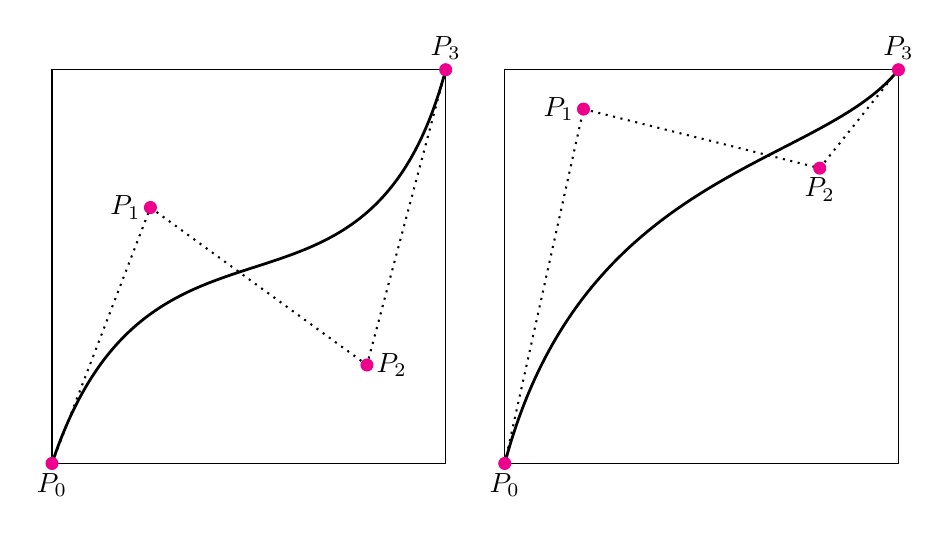
\begin{tikzpicture}[x=5cm,y=5cm]
\draw (0,0) -- (1,0) -- (1,1) -- (0,1) -- (0,0); 
\draw[dotted,line width=.75pt] (0,0) -- (0.25,0.65); 
\draw[dotted,line width=.75pt] (0.25,0.65) -- (0.8,0.25); 
\draw[dotted,line width=.75pt] (1,1) -- (0.8,0.25); 

\draw[line width=1pt] (0,0) .. controls (0.25,0.75) and (0.8,0.25) .. (1,1);

\draw [magenta,fill=magenta] (0,0) node[below,black]{$P_0$} circle (.5ex); 
\draw [magenta,fill=magenta] (0.25,0.65)node[left,black]{$P_1$}  circle (.5ex); 
\draw [magenta,fill=magenta] (0.8,0.25) node[right,black]{$P_2$}  circle (.5ex); 
\draw [magenta,fill=magenta](1.0,1.0) node[above,black]{$P_3$}  circle (.5ex); 

\draw (1.15,0) -- (2.15,0) -- (2.15,1) -- (1.15,1) -- (1.15,0); 
\draw[dotted,line width=.75pt] (1.15,0) -- (1.35,0.9); 
\draw[dotted,line width=.75pt] (1.35,0.9) -- (1.95,0.75); 
\draw[dotted,line width=.75pt] (1.95,0.75) -- (2.15,1); 
\draw[line width=1pt] (1.15,0) .. controls (1.35,0.75) and (1.95,0.75) .. (2.15,1);
\draw [magenta,fill=magenta] (1.15,0) node[below,black]{$P_0$} circle (.5ex); 
\draw [magenta,fill=magenta] (1.35,0.9)node[left,black]{$P_1$}  circle (.5ex); 
\draw [magenta,fill=magenta] (1.95,0.75) node[below,black]{$P_2$}  circle (.5ex); 
\draw [magenta,fill=magenta](2.15,1.0) node[above,black]{$P_3$}  circle (.5ex); 
\end{tikzpicture}
\caption{Kubische Bézierkurven für unterschiedliche $P_1$ und $P_2$}\label{fig:bez}
\end{figure}

CSS~3 bietet dem Nutzer mit dem Schlüsselwort \texttt{cubic-bezier($x_1$,$y_1$,$x_2$,$y_2$)} die Möglichkeit an, eine eigene Transition zu erstellen. Die vier Pflicht-Parameter stehen dabei für die $x$- und $y$-Koordinaten der Punkte $P_1$ und $P_2$ innerhalb des Einheitsraumes (0,0) -- (1,1), die Punkte $P_0$ und $P_3$ sind dadurch definiert.

\section{Erstellung der TikZ-Grafik}

Für meine Studenten wollte ich gern visualisieren, welche Auswirkungen unterschiedliche $P_1$ und $P_2$ Werte auf die erstellte Transition haben. Unter \LaTeX\ gibt es dabei verschiedene Möglichkeit, denn sowohl PSTricks als auch MetaPost und TikZ können Bézierkurven erzeugen. Ich habe mich für TikZ entschieden, da ich mich damit im Vergleich zu PSTricks und MetaPost am besten auskenne 
und auch im WWW jede Menge Ressourcen dazu verfügbar sind. So gelang es auch, die folgende Grafik in wenigen Minuten zu erstellen, passende Suchbegriffe waren natürlich die Voraussetzung. 

Listing \ref{lis:beza} zeigt den Quellcode von Abbildung \ref{fig:beza} und soll nun kurz beschrieben werden. Ich beginne mit einem \verb|\grid|, um bei den folgenden Schritten einen besseren Überblick zu haben. Hinweis: Bei einer Verringerung der Schrittweite des Grids auf acht Zentimeter braucht man auch keinen Polygonzug um die Grafik zu legen, wenn man einen Rahmen um die Zeichnung haben möchte. 

Die anschließenden zwei \verb|\draw| Befehle zeichnen die gepunkteten Hilfslinien und den Bezier-Spline, gefolgt von vier \verb|\draw|-Befehlen, die die kleinen Kreise an den Punkten mit ihren Labels setzen. \clearpage

\begin{lstlisting}[language={[LaTeX]TeX},morekeywords={draw,controls,very,black,gray,thin,grid,magenta,dotted,left,right,above,line,width,%
and,tikzpicture,fill,node,below,step,circle},basicstyle=\ttfamily\footnotesize,caption={Quellcode für Abbildung \ref{fig:beza}},label={lis:beza}]
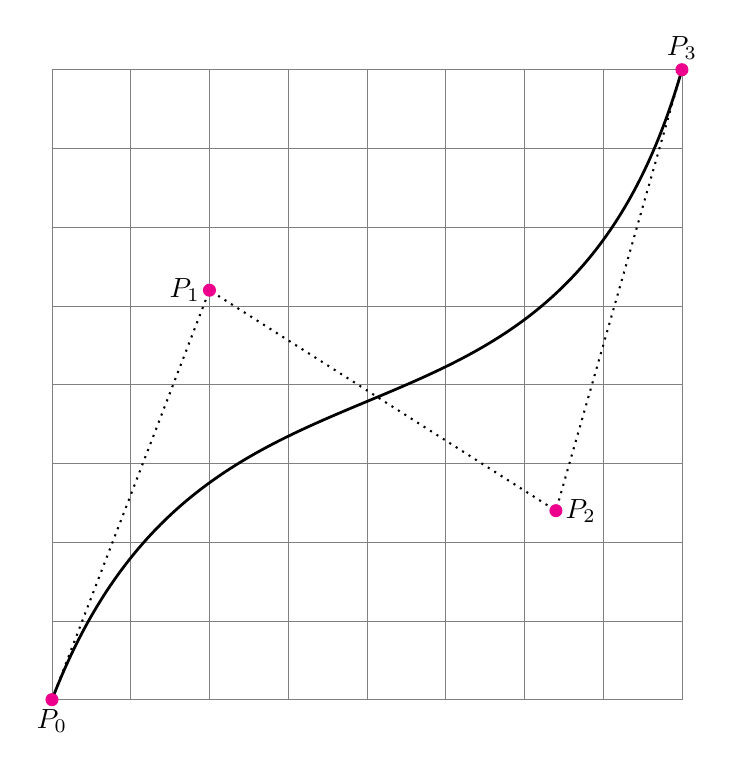
\begin{tikzpicture}[x=8cm,y=8cm]
\draw[step=1cm,gray,very thin] (0,0) grid (1,1);

\draw[dotted,line width=.75pt] (0,0) -- (0.25,0.65) -- (0.8,0.3) -- (1,1);  
\draw[line width=1pt] (0,0) .. controls (0.25,0.65) and (0.8,0.3) .. (1,1);

\draw [magenta,fill=magenta] (0,0) node[below,black]{$P_0$} circle (.5ex); 
\draw [magenta,fill=magenta] (0.25,0.65)node[left,black]{$P_1$}  circle (.5ex); 
\draw [magenta,fill=magenta] (0.8,0.3) node[right,black]{$P_2$}  circle (.5ex); 
\draw [magenta,fill=magenta](1.0,1.0) node[above,black]{$P_3$}  circle (.5ex); 
\end{tikzpicture}
\end{lstlisting}

\begin{figure}[h]
\centering
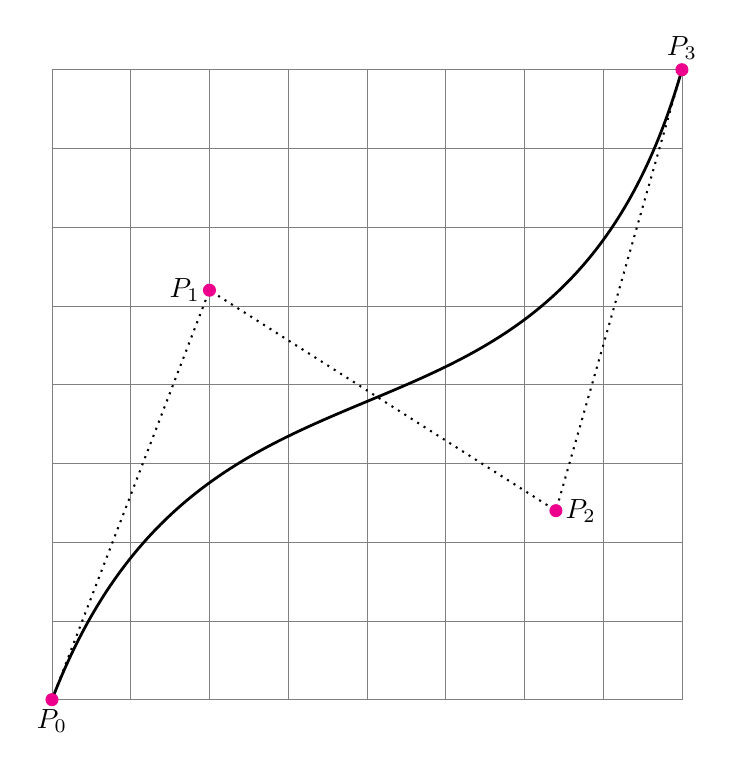
\begin{tikzpicture}[x=8cm,y=8cm]
\draw[step=1cm,gray,very thin] (0,0) grid (1,1);

\draw[dotted,line width=.75pt] (0,0) -- (0.25,0.65) -- (0.8,0.3) -- (1,1);  
\draw[line width=1pt] (0,0) .. controls (0.25,0.65) and (0.8,0.3) .. (1,1);

\draw [magenta,fill=magenta] (0,0) node[below,black]{$P_0$} circle (.5ex); 
\draw [magenta,fill=magenta] (0.25,0.65)node[left,black]{$P_1$}  circle (.5ex); 
\draw [magenta,fill=magenta] (0.8,0.3) node[right,black]{$P_2$}  circle (.5ex); 
\draw [magenta,fill=magenta](1.0,1.0) node[above,black]{$P_3$}  circle (.5ex); 
\end{tikzpicture}
\caption{Kubische Bézierkurve}\label{fig:beza}
\end{figure}\clearpage

\section{Erstellung der Animation}

Nachdem die Grafik jetzt grundsätzlich fertig ist, gilt es, sie zu animieren. Ich habe mich dabei für eine \LaTeX-interne Lösung mittels \texttt{animate}-Paket entschieden. Dieses Paket bietet für die Erzeugung von Animationen verschiedene Möglichkeiten. Neben der Nutzung extern erzeugter Grafiken (egal ob in Form von einzelnen Dateien oder als Teil eines Multipage-Formats wie PDF) können die animierten Inhalte auch direkt in der \LaTeX-Datei erzeugt werden. Im folgenden sollen beide Ansätze an unserem Beispiel vorgestellt werden.

\subsection{Nutzung externer Dateien}

Abbildung \ref{lis:paramcode} zeigt den Quellcode der TikZ-Grafik, hervorgehoben sind die Bereich, die für die Animation verändert werden müssen. Im folgenden wird zwar nur der $y$-Parameter von $P_1$ animiert, das Beispiel lässt sich aber einfach um $x$ bzw. die Animation von $P_2$ erweitern.

\begin{figure}[h]\centering
\fbox{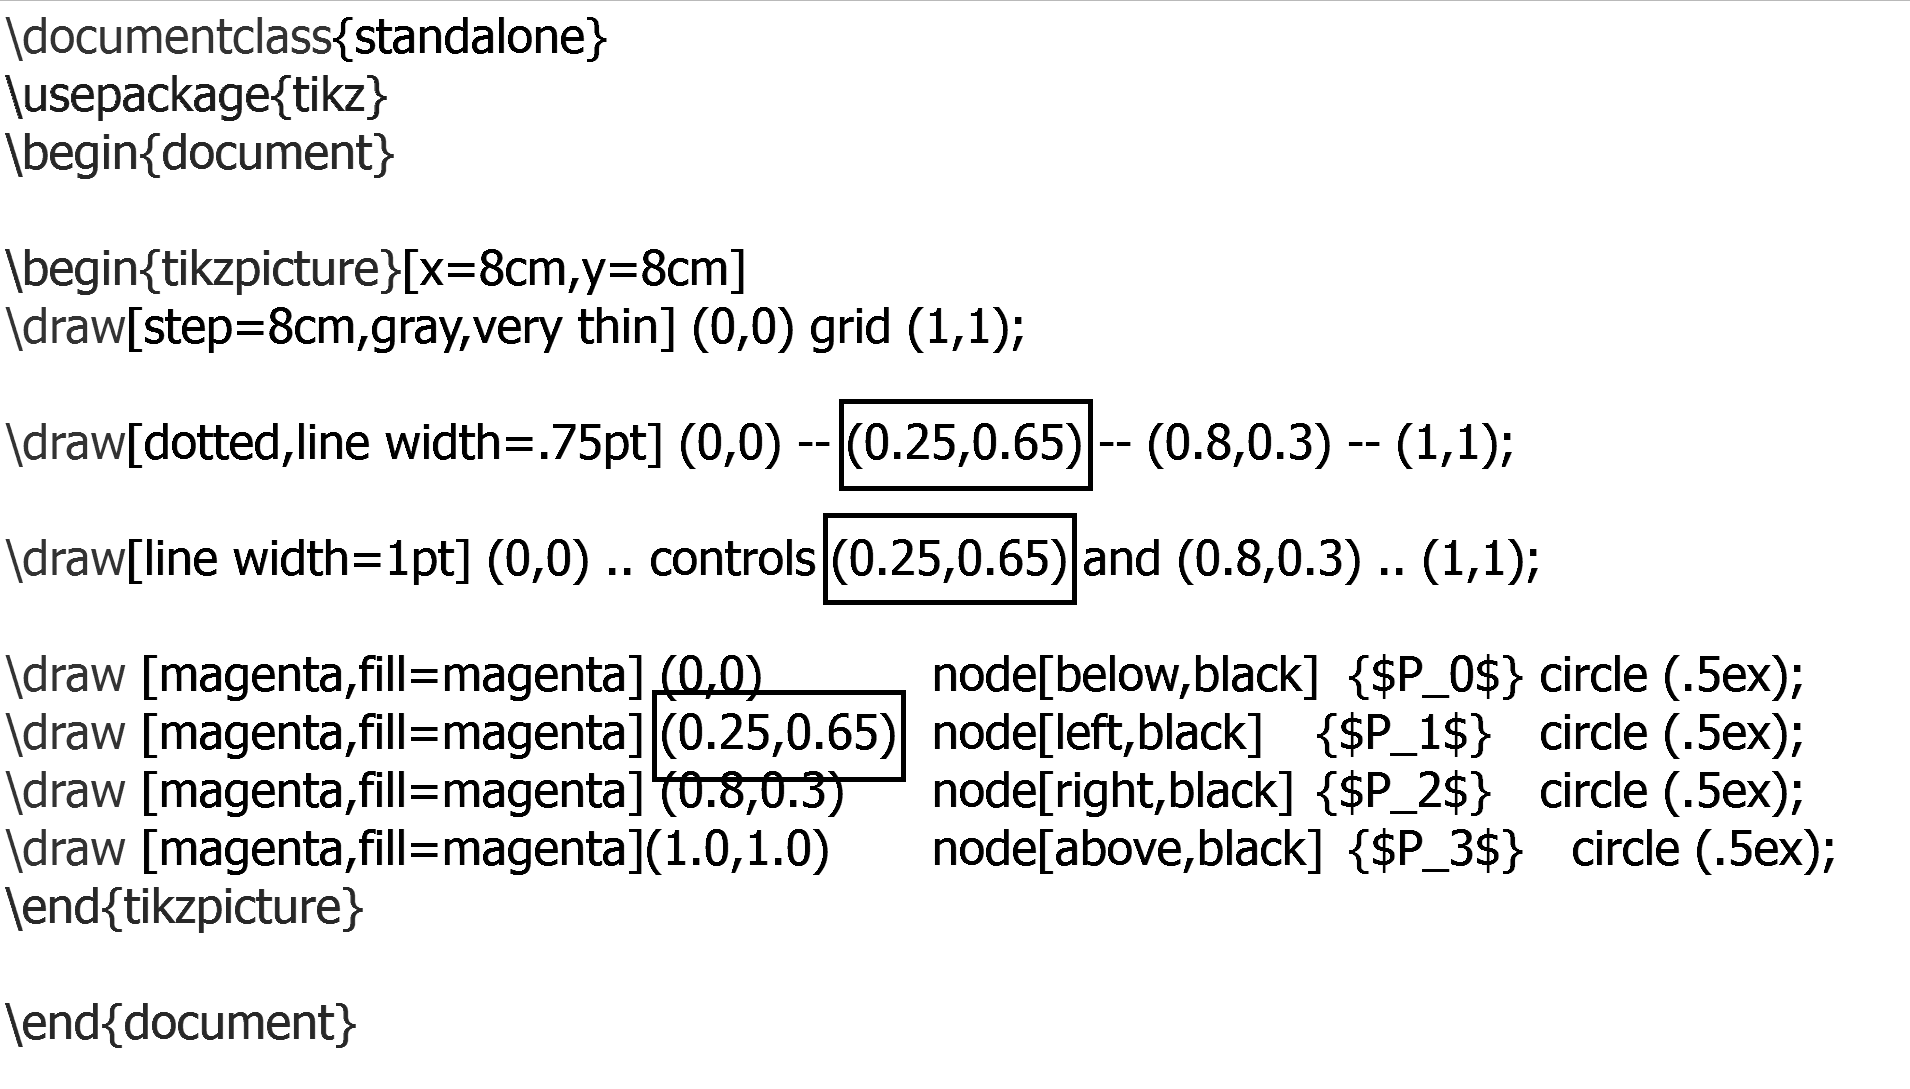
\includegraphics[width=\textwidth]{exttodo}}
\caption{Zu parametrisierende Bereiche des Quell-Codes}\label{lis:paramcode}
\end{figure}

Für die Erstellung der Animationsdatei nutze ich Python, für mich eine der am leichtesten zu lernenden Skript-Sprachen. Im ersten Schritt werden die benötigten Dateien vorbereitet.

\begin{description}
\item[extern.tex] Diese Datei enthält nur die eigentliche TikZ-Grafik. Der Wert für die $y$ Koordinate von $P_1$ wird aber durch \enquote{@@} getauscht, da dieser im folgenden in einer Schleife ausgetauscht wird. Siehe Listing \ref{lis:externtex}
\item[externAnim.tex] Diese Datei enthält das \LaTeX-Gerüst, in das wir im nächsten Schritt die erzeugten Grafiken per \verb|\input| laden. Siehe Listing \ref{lis:externanim}
\end{description}


\begin{lstlisting}[language={[LaTeX]TeX},morekeywords={draw,controls,very,black,gray,thin,grid,magenta,dotted,left,right,above,line,width,%
and,tikzpicture,fill,node,below,step,circle},basicstyle=\ttfamily\footnotesize,caption={Vorlage für die TikZ-Grafik mit \enquote{@@} Platzhaltern},label={lis:externtex}]
\begin{tikzpicture}[x=8cm,y=8cm]
\draw[step=8cm,gray,very thin] (0,0) grid (1,1);

\draw[dotted,line width=.75pt] (0,0) -- (0.25,@@) -- (0.8,0.3) -- (1,1);  
\draw[line width=1pt] (0,0) .. controls (0.25,@@) and (0.8,0.3) .. (1,1);

\draw [magenta,fill=magenta] (0,0) node[below,black]{$P_0$} 	circle (.5ex); 
\draw [magenta,fill=magenta] (0.25,@@) 	node[left,black]{$P_1$} circle (.5ex); 
\draw [magenta,fill=magenta] (0.8,0.3) node[right,black]{$P_2$} circle (.5ex); 
\draw [magenta,fill=magenta](1.0,1.0) node[above,black]{$P_3$} circle (.5ex); 
\end{tikzpicture}
\end{lstlisting}


\begin{lstlisting}[language={[LaTeX]TeX},morekeywords={draw,controls,very,black,gray,thin,grid,magenta,dotted,left,right,above,line,width,%
and,tikzpicture,fill,node,below,step,circle},basicstyle=\ttfamily\footnotesize,caption={\LaTeX-Datei für die Einbindung der erzeugten Datei},label={lis:externanim}]
\documentclass{scrartcl}
\usepackage[paperwidth=10cm,paperheight=10cm,left=0cm,%
right=0cm,top=0cm,bottom=0cm]{geometry}
\usepackage{tikz}
\begin{document}

\input{generated}

\end{document}
\end{lstlisting}

Im nächsten Schritt wird der Python-Code ausgeführt, der in Listing \ref{lis:python} abgedruckt ist. Die ersten sechs Zeilen Zeilen definieren nur eine Funktion, um die Laufweite der später folgenden Schleife zu definieren. Im Anschluss daran wird unsere Template-Datei in die String-Variable \enquote{template} geladen, damit wir im nächsten Schritt die Ersetzungen vornehmen können.


\lstinputlisting[language={Python},caption={Python-Code zur \LaTeX-Erzeugung},label={lis:python}]{generateTikZ.py}

Im letzten Schritt schließlich wird a) eine Datei \enquote{generated.tex} für das Schreiben von Daten geöffnet, b) die Sequenz von 0.1 bis 0.9 in Schritten von 0.05 durchlaufen und c) für jeden dieser Schritte \enquote{@@} in der \enquote{generated.tex} durch den aktuellen Wert der Schleifenvariablen ersetzt. 

Nach dem Lauf dieses Skripts sollte in unserem Arbeitsverzeichnis die \enquote{generated.tex} zu finden sein, die 17 individuelle TikZ-Grafiken enthält. \enquote{externAnim.tex} sollte jetzt problemlos mit z.\,B. \texttt{pdflatex} übersetzbar sein. Eingebunden wird die Datei in ein \LaTeX-Dokument wie folgt:

\begin{center}
\verb|\animategraphics[loop]{5}{externAnim}{}{}|
\end{center}

\enquote{loop} weist den PDF-Viewer\footnote{Ich empfehle Adobe Acrobat, andere Viewer bieten eventuell keine \texttt{animate} Unterstützung.} an, die Animation wiederholt abzuspielen. \enquote{5} steht für die Zahl der Bilder pro Sekunde, die abgespielt werden sollen. Hierbei ist zu beachten, dass höhere Bildraten auch mehr Ressourcen des Rechners erfordern können. \enquote{externAnim} ist der Name der PDF-Datei, die unsere Einzelbilder enthält. Die beiden letzten Parameter dienen der Angabe, welche Bilder aus der Datei geladen werden sollen. In unserem Beispiel sollen alle Bilder dargestellt werden, daher können beide Parameter leer bleiben. Für mehr Informationen siehe die Dokumentation des \texttt{animate} Pakets.

\subsection{Interne Animation}

Listing \ref{lis:inline} auf der nächsten Seite zeigt ein Beispiel, wie mit den internen Funktionen des \texttt{animate} Pakets Animationen 
werden können, ohne auf externe Programme zurückgreifen zu müssen.

Die \texttt{tikzpicture} Umgebung wird in eine \texttt{animateinLine}-Umgebung und einen \texttt{multiframe}-Befehl eingebettet. Die \texttt{animateinLine} Umgebung bekommt als Parameter die Anzahl der Bilder pro Sekunde, der \texttt{multiframe}-Befehl die Anzahl der zu erstellenden Bilder und die Definition einer Zähler-Variablen.

Das \enquote{R} von \enquote{Ry} steht dabei für Gleitkomma-Zahlen, das \texttt{animate}-Paket bietet Unterstützung für weitere Datentypen wie Integer oder \LaTeX-Dimensionen.  In diesem Beispiel läuft der Zähler ebenso wie im extern animierten Beispiel für 17 Bilder von 0.1 in Schritten von 0.05. In der Datei wird diese Zähler-Variablen dann über \verb|\Ry| verwiesen. 

\lstinputlisting[language={[LaTeX]TeX},morekeywords={draw,controls,Ry,animateinLine, multiframe,very,black,gray,thin,grid,magenta,dotted,left,right,above,line,width,%
and,tikzpicture,fill,node,below,step,circle},basicstyle=\ttfamily\footnotesize,caption={\LaTeX-Datei für die Erstellung der internen Animation},label={lis:inline}]{inlineAnimation.tex}

\section{Fazit}

Das \texttt{animate} Paket bietet sehr interessante Möglichkeiten, interne und externe Animationen für \LaTeX-Dokumente zu erstellen. Zur Anzeige ist man aber vermutlich auf Adobe Reader angewiesen, da die JavaScript-Unterstützung bei alternativen PDF-Betrachtern oftmals rudimentär -- wenn überhaupt vorhanden -- ist.

Für Anregungen und Anmerkungen bin ich dankbar, die Beispiele zu diesem Artikel und weitere Code-Beispiele für \texttt{animate} finden sich auch auf meiner Homepage unter \texttt{http://uweziegenhagen.de/?s=animate}.

\end{document}